\documentclass{ifacconf}

\usepackage[english]{babel}
\usepackage{graphicx}
\usepackage{natbib}

\usepackage{amssymb,amsmath}
\usepackage{tikz}
\usetikzlibrary{patterns}
\graphicspath{{media/}}

\DeclareMathOperator*{\argmin}{arg\,min}
%===============================================================================

\begin{document}
\begin{frontmatter}

\title{On the new Algorithm for Solving Continuous Cutting Problem}

\author[urfu]{Petunin A.A}
\author[urfu]{Polishuk E.G.}
\author[urfu]{Ukolov S.S}

\address[urfu]{Ural Federal University, Yekaterinburg, Russia}

\begin{abstract}                % Abstract of not more than 250 words.
The problem of tool path optimization
for CNC thermal cutting machines is considered
along with its classification.
A new approach to solving
Continuous Cutting Problem
is proposed
based on local optimization
using Fermat principle
and Variable Neighbourhood Search approach,
which automatically takes
Precedence Constraint into account,
that is crucial for generating
correct CNC programs
due to technological features
of modern CNC cutting equipment.
\end{abstract}

\begin{keyword}
CNC machine; thermal cutting;
tool path optimization;
CCP; GTSP;
Fermat principle;
Variable Neighbourhood Search
\end{keyword}

\end{frontmatter}

\section{Introduction}

The problem of cutting tool path optimization
is one of the applied optimization problems arising
in the design of control programs for CNC plate cutting machines,
see \cite{Dewil2016Nov}.
The cost or time spent is typically used
as objective function to optimize,
see
\cite{Makarovskikh2018Feb}.
The control program is generated by special software
(Computer-Aided Manufacturing, CAM-system)
just after another well-known optimization problem
has been solved,
i.e. the problem of nesting
(optimal placement of parts to manufacture on the plate),
see \cite{huang2009optimal},
\cite{sherif2014sequential}.
The task is to minimize the consumption of sheet material
to produce the parts of known shapes, sizes and quantity.

The process of figure plate cutting with a CNC machine includes
the following activities:
\begin{itemize}
    \item{Pierce point} (cutting start)
    \item{Actual cutting}
    \item{Turning the cutter off} (cutting end)
    \item{Linear movement from end of cut to start of next cut} (air move)
\end{itemize}

\begin{figure}[b]
    \begin{center}
        \tikz[scale=0.5, transform shape]{
            \tikzstyle{part}=[pattern=north east lines, pattern color=gray,even odd rule]
            \tikzstyle{cutting}=[thick,draw=red,>->|,>=stealth]
            \tikzstyle{air move}=[thick,draw=blue,->,>=stealth]
            \tikzstyle{cutdir}=[cutting,double,->]
            \draw[cutting,part,rounded corners=2mm]
                (0, 0) ellipse (3 and 2)
                (-2, -1) rectangle (2, 1);
            \draw[cutting]
                (-2, 0) +(-45:0.5) coordinate(startA) to[bend left] +(0,0) to[bend left] +(45:0.5) coordinate(endA);
            \draw[cutting]
                (0, 2) +(135:0.5) coordinate(startB) to[bend right] +(0,0) to[bend right] +(45:0.5) coordinate(endB);
            \draw[cutting,part]
                (7, -1) ellipse (3 and 2);
            \draw[cutting]
                (7, 1) +(135:0.5) coordinate(startC) to[bend right] +(0,0) to[bend right] +(45:0.5) coordinate(endC);
            \draw[cutdir] (10.2,-0.5) -- node[sloped, above]{cutting direction} ++(0,-1);
            \draw[cutdir] (-3.2,-0.5) -- node[sloped, above]{cutting direction} ++(0,+1);
            \draw[cutdir] (1.8,0.5) -- ++(0,-1);
            \draw
                (-3, -3) circle(0.05) coordinate(M0) node[below] {$M_0$: Start of control program}
                (startA) circle(0.1) node[right] {$M_1$: Pierce point}
                (endA) node[right] {$M_1^*$: End of cut}
                (startB) circle(0.1) node[above left] {$M_2$: Pierce point}
                (endB) node[above right] {$M_2^*$: End of cut}
                (startC) circle(0.1) node[above right] {$M_3$}
                (endC) node[right] {$M_3^*$}
                (7, -3) node[below] {Part boundary / cutting segment};
            \draw[air move] (M0) -- (startA);
            \draw[air move] (endA) -- (startB);
            \draw[air move] (endB) -- node[sloped, below] {Air move} (startC);
            \draw[air move] (endC) -- (M0);
        }
    \end{center}
    \caption{Example of cutting tool path for two parts and three pierce points} \label{toolpath}
\end{figure}

Control program usually starts with an air move from
some starting point. Fig. \ref{toolpath} represents
the scheme of cutting two parts with three pierce points.
It shows tool path going
along the boundary contours of parts,
while in real life it should be offset to
a half cut width in order to preserve parts geometry and sizes.
From the other hand,
most CAM software assume
the path of cutting tool goes
along parts boundaries,
and actual shift is calculated
by CNC machine itself
or special postprocessing software
while converting tool path
from CAM internal representation
to specific CNC machine language.
In the former case,
exact value of cut allowance
is set by CNC machine operator
just before cutting process.
We will further assume
(if not specified otherwise)
that cutting head path is programmed
directly along bounding contours of the parts to cut,
and final tool path contains all the parts contours.

\section{Formalization}

Let us introduce some notation for tool path components.

We denote $A_1, A_2, \dots A_n$ -- two-dimensional shapes
(closed sets)
that are single- or multiple-connected
regions of Euclidean plane
$\mathbb R^2$.
They are bounded by one or several closed curves
(bounding contours)
$C_1, C_2, \dots C_N,
A_i, C_j \subset \mathbb R^2,
i \in \overline{1, n},
j \in \overline{1, N},
n \leqslant N)$.
Objects $A_1, A_2, \dots A_n$
represent plain parts to cut.

Let also define plane area
$B \subset \mathbb R^2$,
the model of
sheet material, from which parts are to be cut out.
In general,
this area can be of arbitrary complex shape
(contain several non-rectangular pieces),
but in context of tool path optimization
we will assume it to be
one closed point set bounded
(as well as a detail) by one outer contour.
The holes
(inner contours) are acceptable either.
We will suppose the nesting
(positon of the parts within $B$)
somehow fixed already,
meeting the condition of
mutual non-inersection.
Some other requirements may also arise
due to specific technlogical features
of CNC equipment used.
Any way,
fixed disposition of
$A_1, A_2, \dots A_n \subset B$
is available to us.

Then
in accordance with \cite{Petunin2015Nov}
we denote $S=MM^*$ -- a cutting segment,
i.e. the path of cutting head
from pierce point $M$
to the corresponding cut end point $M^*$.
In terms of geometry,
cutting segment is a curve at Euclidean plane:
$S \subset \mathbb R^2,
M(x,y) \in \mathbb R^2,
M^*(x^*,y^*) \in \mathbb R^2$.
We suppose
the cut direction is defined
in every point of segment $S$.
In case when there are no
closed loops inside segment,
cut direction at each point of segment
is defined uniquely by the starting
point of segment $M$
(pierce point).
Tool path can contain closed loops
not only as part bounding contours,
but also to improve cutting quality.

Using the notion of cutting segment,
all the CNC machine cutting technics
can be classified as:
\begin{enumerate}
    \item{\textit{Closed contour cutting (standard)}}:
    each segment contains exactly one part contour
    that is cut from start to end
    \item{\textit{Multi-segment cutting}}:
    part contour consists of two (or more) cutting segments
    \item{\textit{Multi-contour cutting}}:
    several part contours are cut at once within one cutting segment
\end{enumerate}

Let's suppose that our parts
($A_1, A_2, \dots A_n$) were cut
using $K$ cutting segments
$S_k = M_kM_k^*, k \in \overline{1, K}$.
Then we define cutting path as tuple
\begin{multline}
    ROUTE =
    \big< M_0, M_1, S_1, M_1^*, M_2, S_2, M_2^*, \dots \\
    M_K, S_K, M_K^*, i_1, i_2, \dots, i_K \big>
  \label{tuple}
\end{multline}
Here $i_1, i_2, \dots, i_K$ is the sequence of segments
$S_1, S_2, \dots S_K$ processing,
$M_0$ -- starting point of control program.
Linear air moves are impicitly defined by the tuple.
In terms of discrete mathematics,
the sequence is a permutation,
i.e. an ordered set of natural numbers $1\dots K$,
that unambiguously maps every
$K \in \overline{1, K}$ to $i_k$.
As noted before,
we assume tool path to go along
bounding contours of parts
and cutting segments to contain all of them:
$$
\bigcup_{j=1}^N C_j \subset \bigcup_{k=1}^K S_k
$$
Modifying cutting path one can
drastically change numerical parameters
of cutting process.
Therefore a number of optimization problems
arise while developing
control programs for CNC cutting machines.
The most popular objective function
is total cutting time.
In case of thermal or
hydrobarasive cutting the following formula applies:
\begin{equation}
    T_{cut} = \frac{L_{on}}{V_{on}} + \frac{L_{off}}{V_{off}} + N_{pt} \cdot t_{pt}
    \label{cut-time}
\end{equation}
Here,
$L_{off}$ is total length of air moves,
$L_{on}$ is total length of cutting segments,
$V_{off}$ is the speed of air move,
$V_{on}$ is the speed of cutting,
$N_{pt}$ is the number of pierce points,
$t_{pt}$ is the time spent in a pierce point,
assuming it is located in the body of sheet.
In some scenarios other kinds of pierce points
can be used
with their own $t_{pt}$ constants.
In that case, equation (\ref{cut-time})
transforms to
\begin{equation}
    T_{cut} = \frac{L_{on}}{V_{on}} + \frac{L_{off}}{V_{off}}
    + \sum_{j=1}^p N_{pt}^j \cdot t_{pt}^j
    \label{piercings}
\end{equation}
Here,
$p$ is a number of pierce point kinds,
$N_{pt}^j$ -- a number of pierce points of kind $j$,
$t_{pt}^j$ -- time to pierce point of kind $j$.
Both in (\ref{cut-time}) and (\ref{piercings}),
$V_{off}$ is a constant dependent on CNC machine used.
Value of $V_{on}$ is to be determined along with
control program development
concerning cutting technology to use
and parameters of sheet material
(including its thickness).
Thus defined $V_{on}$
is often assumed to be a constant value,
but in practice
actual cutting speed depends on
many technological features as well as
control program itself.
Additional research is required in this area,
some results can be found in
\cite{Tavaeva2017May},
\cite{tavaeva2015definition},
but this is beyond the scope of this article.

Total cost of cutting is another very important
objective function,
especially from economical point of view.
This is rather complex indicator dependent on
electric power consumption,
expendables,
CNC machine maintenance
as well as other operational expenses.

Note that in general cutting cost is not
proprtional to cutting time,
since it also depends on cutting modes.
It can be estimated like in (\ref{cut-time}):
\begin{equation}
    F_{cost} = L_{on}\cdot C_{on} + L_{off}\cdot C_{off} + N_{pt} \cdot C_{pt}
    \label{cut-cost}
\end{equation}
Where
$C_{on}$ is the unit cost of cutting,
$C_{off}$ is that of air move and
$C_{pt}$ is the cost of a piercing a point,
while $L_{on}, L_{off}$ and $N_{pt}$
make the same sence as in (\ref{cut-time}).
Exact values of unit costs
$C_{on}, C_{off}$ and $C_{pt}$
depend on CNC equipment, cutting technology,
sheet material and its thickness.
This dependency is usually summarized
in tabular form or even analitically.

In its turn,
the task of finding appropriate unit costs
$C_{on}, C_{off}$ and $C_{pt}$
for specific equipment and material
is  low-studied itself.
\cite{Tavaeva2015Nov} contains some data concerning this problem
for cutting carbon and stainless steel
as well as aluminium and its alloys
with laser CNC machine ByStar 3015.

When different pierce technologies are used,
(\ref{cut-cost}) becomes
\begin{equation}
    F_{cost} = L_{on}\cdot C_{on} + L_{off}\cdot C_{off}
    + \sum_{j=1}^p N_{pt}^j \cdot C_{pt}^j
    \label{piercings-cost}
\end{equation}
using $C_{pt}^j$ for
cost of piercing of kind $j$.

In any case,
the value of above objective function
depends entirely on the tuple (\ref{tuple})
elements,
i.e. the cutting path.
In detail,
the geometry of cutting segments
$S_1, S_2, \dots S_K$ gives us
total cutting length $L_{on}$,
while points $M_0, M_1, M_1^*, \dots M_K, M_K^*$
with permutation $i_1, i_2, \dots i_K$
describe air moves hence their total length $L_{off}$.

Therefore,
mentioned above problems
of cutting path optimizations may be
stated as minimization of some objective function $F$,
defined on set $G$ of addmisible tuples (\ref{tuple}):
\begin{equation}
    F(ROUTE) \to \min_{ROUTE \in G}
    \label{minimize}
\end{equation}
As tuple contains both
cutting sequence
$i_1, i_2, \dots i_K$
and cutting start and end points
$M_kM_k^*, k \in \overline{1, K}$,
the latter located on the Euclidean plane $\mathbb R^2$,
general optimization problem (\ref{minimize})
is a very complex
continuous-discrete optimization problem,
even with significant restrictions imposed
on admissible segments
$S_1, S_2, \dots S_K$.

This leads to the fact that
there are no general algorithms for solving the problem (\ref{minimize})
described in the scientific literature.
Nevertheless,
some narrow classes of problems
exist,
that allow efficent optimization algorithms to be developed,
see \cite{dewil2012heuristics}.
We mention four such classes:

\begin{enumerate}
    \item \textbf{Continuous Cutting Problem (CCP)}:
    the cutter head visits each contour to be cut once.
    The tool can engage the contour at any point on its perimeter,
    but must cut the entire
    contour before it travels to the next contour.
    Accordingly, the same point must be used for
    entry and exit the contour.
    In terms of cutting techniques CCP implies the standard one.
    With no constraints on the pierce points,
    problem (\ref{cut-time}) reduces to finding minimal
    air move distance $L_{off}$,
    which is equivalent to the classical metric TSP
    (Travelling Salesman Problem).
    A significant part of the publications is devoted precisely
    to the solution of this particular optimization problem

    \item \textbf{Endpoint Cutting Problem (ECP)}:
    the tool can enter and exit contours only at some
    predefined points on the boundary.
    However, it may cut the contour in sections,
    or stated otherwise: a contour can be pre-empted.
    This approach reduces the complexity of full problem
    by discretiztion of possible pierce point set and therefore
    contour entry points as well.
    Set of contour exit points is equal to that of
    entry points, however,
    contour exit point is not neccesary
    a point of cutting end
    (where cutting head is switched off),
    because cutting can continue to another contour.

    \item \textbf{Generalized Traveling Salesman Problem \\ (GTSP)}:
    the tool path visits each contour to be cut once
    and the tool can engage the contour only
    at some predened points on the boundary.
    This is a special case for CCP and ECP problems.

    \item \textbf{Segment Continuous Cutting Problem (SCCP)}:
    cutter head visits each segment to be cut once.
    The tool can engage the segment at any point,
    but must cut the entire segment before it travels to the next segment,
    see \cite{Petunin2015Nov}.

    Note: $CCP \subset SCCP$.

    This case uses the concept of basic cutting segment
    $B^S$, the part of full cutting segment
    $S = MM^*$ with lead-in and lead-out excluded.
    Unlike full cutting segments,
    basic ones doesn't assume cutting direction,
    containig only geometrical data.
    When standard cutting technique is used only,
    the set of basic segments $\bigcup B^S = \bigcup C_i$
    (the set of bounding contours).

\end{enumerate}

First classification of tool path routing problems
was proposed in:
\cite{Hoeft1997Sep}.

Most publications on the area explore GTSP problem
and develop appropriate algorithms,
see for example \cite{Helsgaun2015Sep}.
Its main advantage is that most methods
of standard GTSP problems can be applied,
only some additional constraints should be
taken into account,
for instance -- precedence constraint.

It imposes restrictions on the order of
segment processing
$I = (i_1, i_2, \dots i_K)$.
Modern CNC cutting equipment cannot guarantee
positioning of cutting head inside the contour
that is alredy cut,
because the part can freely move
(or even drop)
after it is detached from the sheet.
To cope with this,
the following rules must be obeyed:

\begin{enumerate}
    \item{If one or more inner contours (holes) are inside outer one,
    then they all must be cut before cutting of outer contour starts
    }
    \item{If some other part is placed inside
    inner contour of a part,
    the former one must be cut before the latter.
    Rule 1 applies either.}
\end{enumerate}
These rules are the precedence constraint
for the permutation
$I = (i_1, i_2, \dots i_K)$.
In other words:
\begin{enumerate}
    \item{If permutation
    $I = (i_1, \dots i_k, \dots i_K)$
    contains outer contour $i_k$,
    all its corresponding inner contours $i_x$
    must apeear before $i_k$.
    }
    \item{If permutation
    $I = (i_1, \dots i_k, \dots i_K)$
    contains inner contour $i_k$
    and there is some outer contour
    of another part $A_l, l \in \overline{1,n}$
    inside it,
    that outer contour must precede $i_k$
    in permutation $I$}
\end{enumerate}

Both the precedence constraint
and pierce point constraints
are of static nature,
that is they are completely defined by
the nesting the parts on the sheet,
CNC equipment and material used
and are not affected by the elements
of tuple itself.
In terms of tool path
(\ref{tuple}),
some of permutations
$I = (i_1, i_2, \dots i_K)$
are just forbidden.
Of many recent papers
on GTSP cutting optimization algorithms,
we note
\cite{Vicencio2014Sep},
\cite{yu2014route},
\cite{Karapetyan2012Jun},
\cite{Yang2010},
\cite{d2003tool}.

A number of technological features of modern CNC equipment
impose a few other constraints on
pierce points and segment cutting order.
But unlike mentioned above,
these constraints are dynamic,
they depend on the preceding elements
of tuple (\ref{tuple})
and caused by
thermal deformations of sheet material.
It is rather difficult to get comprehensive
equation for such constraints,
see \cite{chentsov2013dynamic}, \cite{chentsov2015model} for approaches.
These constraints, however,
are also beyond the scope of the paper.

Another class of cutting path optimization problems exists,
named \textbf{Intermittent Cutting Problem (ICP)}.
This is the most general version of the problem
where contours can be pre-empted and there is
no restriction on the points that can be used for entry or exit.
It is roughly equivalent to problem (\ref{minimize}).

\section{Dual relaxation for CCP}
As stated above,
we assume cutting goes along part boundaries
$S_i = C_i, \forall i=\overline{1, k}$
and piercing point $M_i$ is always equal to
cutter off point,
so as both lay on the contour:
$M_i \equiv M_i^* \in C_i, \forall i = \overline{1, k}$.

Tool path starting point $M_0$ is also fixed.

Finally,
to suit most modern CNC cutting equipment,
every closed contour $C_i \equiv S_i$
is assumed to be
a finite set of circular arcs
and straight line segments.
It is tempting to reduce
CCP to
Touring Polygons Problem
(see \cite{Qin2017Nov} for example),
but we consider more general problem.

In our notations Continuous Cutting Problem is to find:
\begin{enumerate}
  \item Positions of $k$ piercing points $M_i \in C_i$
  \item Order of contours $C_i$ processing,
  i.e. the permutation of $k$ items
  $I=(i_1, i_2, \dots, i_k),
    i_j \in \overline{1,k}, \forall j \in \overline{1,k}$
\end{enumerate}
Objective function of cutting time (\ref{cut-time})
in our case can be simplified to total length of air movements
$$
\mathcal L = \sum_{j=0}^k |\overrightarrow{M_{i_j} M_{i_{{j+1}}}}|
$$
$$
\mathcal L \to \min
$$
where we suppose
$M_{i_0} = M_{i_{k+1}} = M_0$
in sake of brevity.

This problem is often
reduced to GTSP
(Generalized Traveling Salesman Problem)
by means of
discretization of contours $C_i$
with some step $\varepsilon$.
Finding piercing point $M_i$
becomes a discrete optimization problem
of choosing among finite number of
candidates.
But we are to solve
problem of both discrete and
continuous optimiztion.

In addition,
the \textit{Precedence Constraint}
is considered.
For CCP we can state it in a simpler form:
when some contour is inside another one,
the former must be cut
before the latter
$$
\tilde C_a \subset \tilde C_b
\Rightarrow
i_a < i_b
$$
where we denote
$\tilde C_i$ a 2D figure,
bounded by $C_i$.

Thus stated Precedence Constraint
limits the feasible subset of permutations
$I=(i_1, i_2, \dots, i_k)$,
that are the part of
complete problem solution (\ref{tuple}).

\subsection{Continuous optimization}
In practice,
the shape of part bounding contours
is limited to a finite set
of straight line segments and circular arcs.
This allows exact solution of
subproblem of optimal
positioning of single pierce point $M_i$,
while others are fixed as well as
processing order
$I=(i_1, i_2, \dots, i_k)$.
$$
\mathcal L \to \min_{M_i}
$$
which in turn means
$$
\sqrt{\overrightarrow{M_i M_{i-1}}^2} +
\sqrt{\overrightarrow{M_i M_{i+1}}^2} \to
\min_{M_i \in C_i}
$$
Simple consideration reveals,
that
if neighbour pierce
point (assumed to be fixed)
lay on both sides of cutting segment
(i.e. line or circle containing the latter),
optimal position is an
inersection of line $M_{i-1}M_{i+1}$
with segment itself
$$
M_i = M_{i-1}M_{i+1} \cap S_i
$$
When neighbours are situated
on the same side,
famous \textit{Fermat principle}
should be applied,
leading to
angle of incidence be equal to the angle of reflection,
as seen on Fig. \ref{fermat}.

\begin{figure}
  \begin{center}
  \tikz[rotate=27,scale=1.3]{
      \draw[thick]
          (0, 0) coordinate(zero) -- (5, 0) coordinate(future) node[right] {$S_i$};
      \fill[black]
          (1.5, 0) circle(0.1) coordinate(middle) node[below right]  {$M_i \equiv M_i^*$}
          (1, 1) circle(0.1) coordinate(from) node[above left] {$M_{i-1}$} ++(-1.5,0) node[above] {$S_{i-1}$}
          (4.5, 2) circle(0.1) coordinate(to) node[above] {$M_{i+1}$} ++(1.5,0) node[below] {$S_{i+1}$};
      \begin{scope}
          \clip (from) circle(1);
          \draw[thick] (from) ++(0, 3) circle(3);
      \end{scope};
      \begin{scope}
          \clip (to) circle(1.5);
          \draw[thick] (to) ++(3, 4) circle(5);
      \end{scope};
      \draw[dashed] (from) -- (middle) -- (to);
      \draw[thin] (4.5, -2) circle(0.062) coordinate(mirror) node[right] {$\hat M_{i+1}$};
      \coordinate (opt) at (intersection of zero--future and mirror--from);
      \draw[thin] (opt) circle(0.1);
      \draw[dotted]
          (mirror) -- (opt)
          (mirror) -- (to);
      \draw[thin] (from) -- (opt) -- (to);

      \draw[->,>=latex,red,thick] (middle) to[bend right] (opt);

  }
  \caption{Applying Fermat principle to find piercing point} \label{fermat}
  \end{center}
\end{figure}

Similar to
\textit{Alternating Least Squares}
(ALS)
method,
the complete process
for positioing all the pierce points
$M_i, i \in \overline{1,k}$
could be called
\textit{Alternative Fermat Principle}
and organized as follow:
\begin{itemize}
  \item Randomly choose initial position $M_i \in C_i, \forall i$
  \item $\forall i \in \overline{1,k}$ find optimal $M_i$ as stated above in constant time $O(1)$
  \item Repeat until all pierce point position $M_i, \forall i$ converge
  (with some predefined accuracy $\delta$)
\end{itemize}

In practice this process also
converges well in $O(k)$ time,
that is why we use it
as one step for complete
procedure of continuous and discrete optimization.

\subsection{Discrete optimization}

Discrete optimization problem
to be solved inside CCP
is to find permutation
$I=(i_1, i_2, \dots, i_k)$,
minimizing total air move length
$$
\mathcal L \to \min_{i_1, i_2, \dots i_k}
$$
Variable Neighborhood Search
(VNS)
over full set of permutations
is used,
see \cite{Hansen2010Mar}.

The general scheme of VNS as applied to CCP:
\begin{enumerate}
  \item $ I \gets random P_k$
  \item $ k \gets 1$
  \item \textbf{while} $k < k_{max}$
  \begin{enumerate}
  \item $ I' \gets \argmin\limits_{I' \in \mathcal N^k(I)} \mathcal L(I')$
  \item \textbf{if} $\mathcal L(I') < \mathcal L(I)$
  \begin{itemize}
      \item $I \gets I'$
      \item $ k \gets 1$
  \end{itemize}
  \item \textbf{else}
  \begin{itemize}
      \item $ k \gets k+1$
  \end{itemize}
  \end{enumerate}
  \item \textbf{end}
\end{enumerate}
Step (a) repeatedly applies
above described continuous
optimization,
actually
$$
\mathcal L(I') = \min_{M_1, M_2, \dots M_k} \mathcal L(M_1, M_2, \dots M_k | I')
$$

To build neighbourhoods
$\mathcal N^k(I)$
of different structures,
various techniques are used.
Only a few of them
can be expressed in terms of
popular metrics.

\begin{itemize}
\item All pairwise permutations of the current one
$I=(i_1, i_2, \dots, i_k)$.
This neighbourhood can be
generated using Levenshtein distance

\item Permutations of three items (contours to cut).
Enumeration of all triple permutations
requires $O(k^3)$ time,
so it was restricted
by permutations with elements
whose pairwise distance is below
some value
(algorithm parameter)

\item In a similar manner,
quadriple permutations are considered,
limited to some pairwise distance

\item Cyclic permutations inside a sequential block of arbitrary length
\item Reversing sequential block of arbitrary length
\item Permutations of two sequential blocks of the same length
\item Cyclic shift of a chain of blocks of the same length
\item About dozen other options for constructing a neighborhood of a permutation $ \mathcal N (I) $
\end{itemize}

When some technique yields
too large neighbourhoods,
it can be easily limited
by simple heuristics,
just as the one used for
triple and quadriple permutations.

Besides,
various options of
Variable Neighborhood Search approach
may be used,
such as
\textit{First Improvement}
(instead of above described \textit{Best Improvement})
or
stochastic point selection.
Performance of these options
is the subject of further research.

\subsection{Precedence constraint}

Described steps of the algorithm
can be considered as one of the solutions
for
\textit{Traveling Salesman Problem}
(TSP)
with quasi-Euclidean city distance.

But cutting tool path optimization
must also take into account a number of
additional constraints,
caused by technological features
of CNC equipment.
Most popular of them is
\textit{Precedence Constraint}.

Luckily, it can be easily accounted
inside proposed algorithm.
To do so,
we start from discarding the contours,
that contains others inside:
\begin{equation}
\big\{
    C_i | \forall j \ne i: C_j \cap \tilde C_i = \varnothing
\big\}
\label{non-outers}
\end{equation}
For that new set of contours
we solve the unconstrained CCP
as described above.
Note, that resulting air move path
\begin{equation}
  \bigcup_{i=0}^{k'} M_i M_{i+1}
\label{path-found}
\end{equation}
intersect \textbf{all}
source contours
$C_i, i \in \overline{1,k}$.

Indeed,
it intersects the contours in (\ref{non-outers})
by construction,
and the others
(outer ones),
because
its start and finish point
$M_0 \equiv M_{k+1}$
is outside all the contours,
and every outer contour
contains at least one contour
(\ref{non-outers}) inside.

Now,
we proceed to the
previously skipped contour $C_i$
without pierce point $M_i$
(i.e. it contains some contours in
(\ref{non-outers}) inside).
We find all the intersection
points $C_i \cap $ (\ref{path-found})
and since there are several such points,
we select \textit{last} one of them
(according to path (\ref{path-found}) direction).

Next, we add all new points $M_i$ found
to path (\ref{path-found}).
This is the solution of original CCP,
considering the
\textit{Precedence Constraint}.
Its length obviously remains the same
during extra point insertion.

The resulting path contains all $k$
piercing points
$M_i, \forall i \in \overline{1,k}$
and point for outer contour
is guaranteed to pass after
the points for its inner ones.

Further,
when solution for partial problem
is optimal
(according to length of air move),
the final solution
is optimal either.
Indeed,
if shorter full path existed,
then one could build solution
for partial problem
by discarding all the contours not in
(\ref{non-outers}) with their piercing points,
preserving total path length.
But it is supposed imposible
for such a solution to exist.

The technique described thus
effectively takes
\textit{Precedence Constraint}
into account while solving CCP.
Moreover,
it reduces the problem space dimension,
leading to lower time requirements.

\section{Numerical experiments}

\begin{figure}
  \resizebox*{0.48\textwidth}{!}{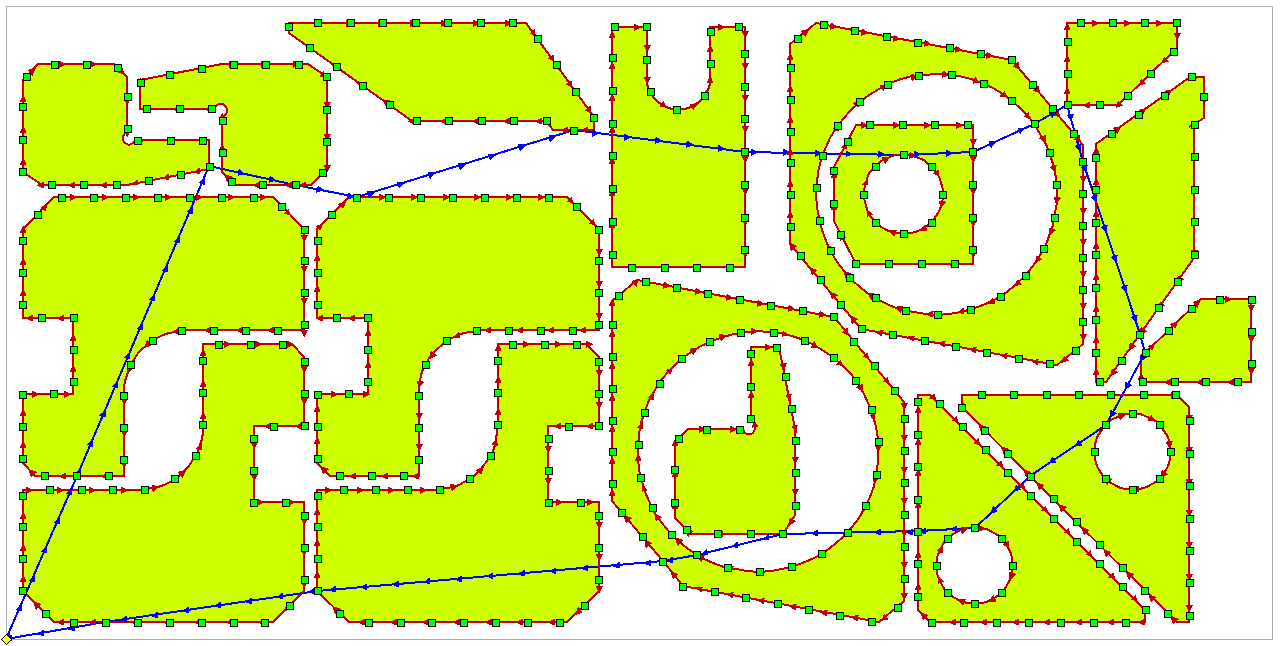
\includegraphics{3211-gtsp.png}}
  \caption{Exact solution of GTSP, Job \#3211}
  \label{gtsp-path}
\end{figure}

From a practical point of view, the proposed algorithm
turns out to be very successful
and finds easily good solutions
despite the lack of mathematical guarantees for this.

In order to confirm this claim
a series of experiments were conducted.
The results of the propsed algorithm
were compared with the ones
of another algorithm,
which is proved to
find the exact solution to the GTSP problem
with the number of contours
(\textit{megalopolices}) no more than 32,
see
\cite{Chentsov2018Jul},
\cite{petunin2014local}.

The comparison results are in the table. \ref {exact-3}.

\begin{table}[h]
  \begin{center}
  \begin{tabular}{l|*{3}{r}}
      Job & \#229 & \#464 & \#3211 \\
      \hline
      \# of parts & 11 & 14 & 17\\
      \# of contours & 12 & 21 & 22 \\
      $L_{on}$, m & 24.609 & 21.717 & 25.051 \\
      \# of GTSP points & 491 & 429 & 493 \\
      GTSP's $L_{off}$, m & 7.729 & 4.743 & 4.557 \\
      Our $L_{off}$, m & 7.727 & 4.706 & 4.536 \\
  \end{tabular}
  \caption{Solution quality comparison}
  \label{exact-3}
  \end{center}
\end{table}

The quality of the constructed
cutting path can be visually compared
on Fig. \ref{gtsp-path} and Fig. \ref{ccp-path}.

Values of $L_{off}$ are in good compliance for two algorihtms used
as well as shapes of the paths themselves.

Dual relaxation finds even slightly shorter tool path,
because it can route cutting head along straight lines
whereas GTSP's tool path is always polygonal
due to preliminary discretization involved.
In other words,
optimal solution for CCP is always a bit shorter
than that of GTSP.

\begin{figure}
  \resizebox*{0.48\textwidth}{!}{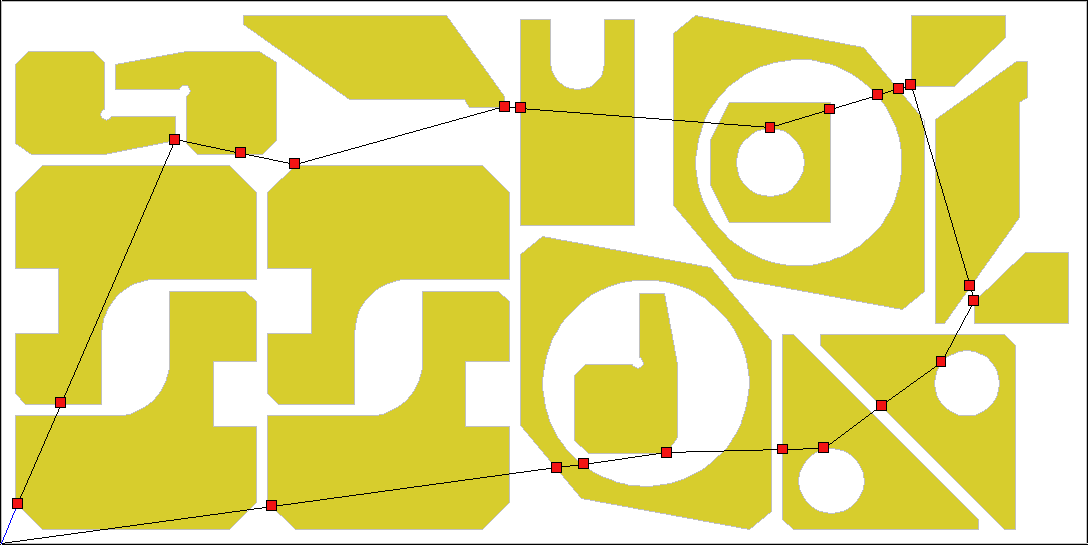
\includegraphics{3211-ccp.png}}
  \caption{Solution of CCP, Job \#3211}
  \label{ccp-path}
\end{figure}

\section{Conclusion}

The new heuristic algorithm
for solving
Continuous Cutting Problem
for CNC cutting machine
is described end evaluated...

\begin{ack}
The work was supported by Act 211 Government of the Russian Federation,
contract \# 02.A03.21.0006
\end{ack}

\bibliography{ccp-vns}             % bib file to produce the bibliography

\end{document}
